\documentclass[class=article,border=5pt,tikz]{standalone}
\usetikzlibrary{calc}

\begin{document}
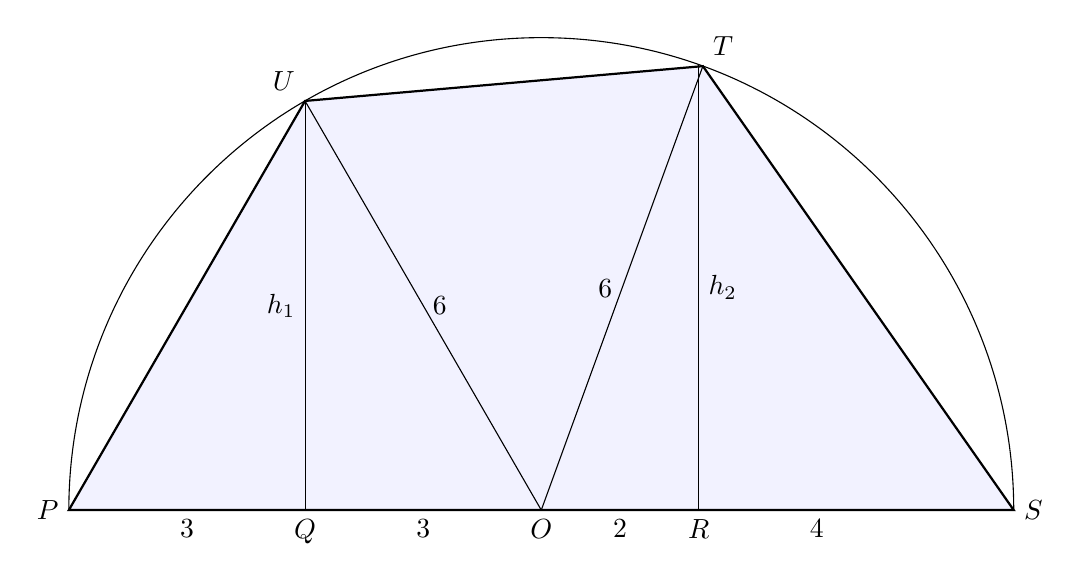
\begin{tikzpicture}
\path (180:6) coordinate (P) (120:6) coordinate (U) (70:6) coordinate (T) (0:6) coordinate (S);
\draw[thick,fill=blue!5] (P) node[left]{$P$} -- (U) node[above left]{$U$} -- (T) node[above right]{$T$} -- (S) node[right]{$S$} -- cycle;
\draw[thin] (P) -- (S) arc(0:180:6) --cycle;
\draw[thin] (-3,0) node[below]{$Q$} -- (-3,{3*sqrt(3)}) node[midway,left]{$h_1$};
\draw[thin] (+2,0) node[below]{$R$} -- (+2,{4*sqrt(2)}) node[midway,right]{$h_2$};
\node[below] at (-4.5,0) {$3$};
\node[below] at (-1.5,0) {$3$};
\node[below] at (+1,0) {$2$};
\node[below] at (3.5,0) {$4$};
\coordinate (O) at (0,0);
\node[below] at (O) {$O$};
\draw[thin] (U) -- (O) node[midway, right] {$6$};
\draw[thin] (T) -- (O) node[midway, left] {$6$};
\end{tikzpicture}
\end{document}
